Learning to classify new categories from different domains is always an interesting and challenging topic in data mining.
Previous empirical and theoretical studies have shown that testing error is positively proportional to the difference between the test and training input distributions \cite{ben2007analysis} \cite{blitzer2008learning}. Therefore, mismatched data distribution can be the major problem for predicting the data from a different domain. Domain adaptation is proposed to solve this problem, transferring the knowledge from source domain to target one. For image recognition tasks, model trained from the source domain is inherently biased as there is no database that includes all the transformations of the objects.

Automatically recognizing the food images is a practical technique in daily life, from which people would benefit in various ways, such as healthy eating and diet control. The properties of the food image makes it a very challenging task for recognition (see Section \ref{sec:bg}).
Recently, Deep Convolutional Neural Network (CNN) shows its potential to replace the shallow features, such as SIFT \cite{lowe1999object}, SURF \cite{bay2006surf} and HOG \cite{dalal2005histograms} etc, in large object recognition tasks \cite{krizhevsky2012imagenet} \cite{zeiler2014visualizing} \cite{simonyan2014very}. Unlike the local feature which presents an shallow interpretation of spatial property, deep CNN can automatically learn top-down hierarchical feature representations. Therefore, deep CNN has been intensively used as the feature extractor for image recognition \cite{farabet2013learning}. As deep feature representation has strong generalization ability, it can compensate for the data bias and be applied for domain adaptation. Fine-tuning the whole network with the pre-trained models on target domain directly has shown some impressive results from previous studies \cite{zeiler2014visualizing} \cite{Chatfield14} \cite{hoffman2013one} \cite{NIPS2014_Zhou}.
However, fine-tuning deep CNNs with limited training data could lead to overfitting which is mostly due to the sampling noise \cite{srivastava2014dropout}.

Even though, it is difficult to obtain a satisfied result for fine-tuning deep CNNs on a small dataset, there is no limitation for training linear shallow models with deep representation from the target domain. Fine-grained feature representation can be obtained by fine-tuning deep CNN on a relatively large source domain and alleviate the distribution bias for target domain \cite{zhang2014part}. Moreover, we find that fine-grained deep representation can also help the shallow classifier learn categories with fewer examples.
So by applying appropriate adaptation strategy, the shallow models can still adapt new categories with fewer examples.

From previous studies, many shallow domain adaptation methods for the image recognition task have been proposed to compensate the dataset bias, assuming that the parameters of the linear classifier for similar categories have certain linear correlation \cite{daume2009frustratingly} \cite{yang2007adapting} \cite{aytar2011tabula}.
%Since the previous methods are limited to either similar categories or requiring many labeled examples, it would be ideal for a method that can learn and predict new categories with just a few labeled training examples.
However, these methods require the target category to be geometrically similar to the source one \cite{aytar2011tabula}. They use shallow feature representation such as HOG or SIFT etc, as the inputs of the linear model. So the inputs of the two categories should be similar and the linear assumption of the parameters can be applied directly for adaptation. But according to our experiments (see Section\ref{sec:da}), this assumption could fail when the representations of two categories are not similar.
Deep CNN can learn fine-grained feature representations and the feature representations of two similar categories are not necessarily to be close to each other. The linear correlation assumption may fail when using the deep representation. We find that even for two similar categories, the parameters of their classifiers is not necessarily to be similar for deep representation (see Section \ref{sec:ft}).

Instead of finding linear correlated parameters for the new category from learned categories, we employ a negative classifier whose parameters are "far away" from any previous learned model parameters. Technically, this negative classifier is trained to classify all examples from learned categories as negative examples (see Figure \ref{fig:wm}). Experiment results show that initialize the new classifier with parameters of this negative classifier (warm start) can achieve better result. The idea of warm start has been widely used for linear optimization problem, where the algorithm iteratively initializes and updates the parameters from the result of previous steps. Previous studies suggest that warm started parameters can achieve better accuracy and fast convergency \cite{yildirim2002warm} \cite{john2008implementation} \cite{zeilinger2011real} \cite{chuwarm}.

\begin{figure*}
  \centering
  % Requires \usepackage{graphicx}
  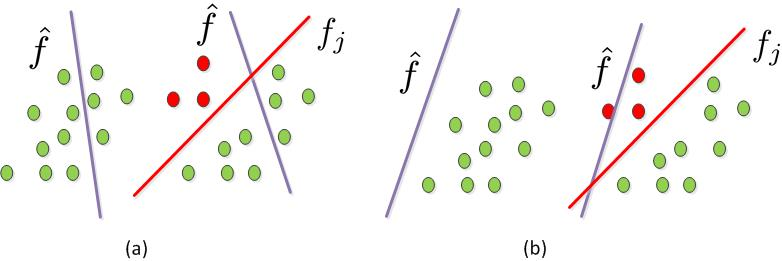
\includegraphics[scale = .6]{fig/domain2.jpg}\\
  \caption{The classifier for class $j$ is initialized with $\hat{f}$ and converged at $f_j$. (a) Conventional adaptation method using the parameters of the learned category and need more training time find good solution for the target category. (b) The parameters from $\hat{f}$ reject all learned categories and can learn faster for the new categories.}
  \label{fig:wm}
\end{figure*}

In this paper, we aim the adaptation problem on a specific area, food recognition. We first obtained a model that can learn 101 kinds of food from deep representation and try to deal with the problem: adapting new foods from other dataset. We propose an incremental adaptive approach that can learn new foods with a few labeled images. There are two main contributions of our work:
\begin{enumerate}
  \item Training deep feature extractor. To generate fine-grained deep representation from food images, we first train the efficient feature extractor by fine-tuning GoogLeNet and achieve the state-of-the-art performance on our source domain, Food-101 dataset. With deep representation, compared to the results training on full dataset, we can achieve similar results while just using a few examples in each category.
  \item Negative classifier for warm start. Warm start new classifier with negative classifier can take advantage of deep representation. Benefitting from warm start parameters in each step, experimental results show that our method can achieve better result. Also our warm started parameters can converge with fewer training iterations.
\end{enumerate}

The rest of this paper is organized as follow: In Section \ref{sec:bg} we introduce the two datasets and discuss some properties about the food recognition task. In order to obtain discriminative representations from images, we fine-tuned GoogLeNet with pre-trained parameters from ImageNet and achieve state-of-the-art performance on our source domain, Food-101 dataset in Section \ref{sec:ft}. We discuss the limitations of some previous adaptation methods and propose our warm start adaptation method for learning new categories in Section \ref{sec:da}.
